\documentclass[journal]{IEEEtran}
\usepackage{cite}
\usepackage{amsmath,amssymb}
\usepackage{graphicx}
\usepackage{booktabs}
\usepackage{adjustbox}
\usepackage{tikz}
\usetikzlibrary{positioning,arrows.meta,shapes.geometric}
\usepackage[hidelinks]{hyperref}
\usepackage{url}
\newcommand{\RKwBmOne}{63.4}
\newcommand{\RKwBmFive}{99.9}
\newcommand{\RKwBmMrr}{0.791}
\newcommand{\RKwDnOne}{53.1}
\newcommand{\RKwDnFive}{87.5}
\newcommand{\RKwDnMrr}{0.675}
\newcommand{\RKwHyOne}{60.0}
\newcommand{\RKwHyFive}{96.2}
\newcommand{\RKwHyMrr}{0.752}
\newcommand{\RSynBmOne}{46.2}
\newcommand{\RSynBmFive}{81.3}
\newcommand{\RSynBmMrr}{0.605}
\newcommand{\RSynDnOne}{48.6}
\newcommand{\RSynDnFive}{81.6}
\newcommand{\RSynDnMrr}{0.628}
\newcommand{\RSynHyOne}{52.7}
\newcommand{\RSynHyFive}{89.6}
\newcommand{\RSynHyMrr}{0.680}
\newcommand{\ROverallBm}{57.7}
\newcommand{\ROverallDn}{51.6}
\newcommand{\ROverallHy}{57.6}
\newcommand{\AccNoAcl}{63.9}
\newcommand{\LeakNoAcl}{87.1}
\newcommand{\TopFiveNoAcl}{100.0}
\newcommand{\AbstNoAcl}{12.3}
\newcommand{\AccPost}{64.3}
\newcommand{\LeakPost}{0.0}
\newcommand{\TopFivePost}{0.0}
\newcommand{\AbstPost}{99.1}
\newcommand{\AccPre}{64.4}
\newcommand{\LeakPre}{0.0}
\newcommand{\TopFivePre}{0.0}
\newcommand{\AbstPre}{75.0}
\newcommand{\KOnePre}{47.4}
\newcommand{\KOnePost}{46.6}
\newcommand{\KTwoPre}{58.4}
\newcommand{\KTwoPost}{57.7}
\newcommand{\KThreePre}{63.6}
\newcommand{\KThreePost}{63.1}
\newcommand{\KTenPre}{64.4}
\newcommand{\KTenPost}{64.3}
\newcommand{\UnauthPairs}{2{,}232}
\newcommand{\AuthPairs}{5{,}196}
\newcommand{\GStdCorr}{67.2}
\newcommand{\GCovEightCorr}{50.0}
\newcommand{\GCovNineCorr}{25.8}
\newcommand{\GStdWrong}{21.2}
\newcommand{\GCovEightWrong}{6.8}
\newcommand{\GCovNineWrong}{0.1}
\newcommand{\GStdAbst}{11.6}
\newcommand{\GCovEightAbst}{43.2}
\newcommand{\GCovNineAbst}{74.2}
\newcommand{\GStdFalse}{80.6}
\newcommand{\GCovEightFalse}{31.1}
\newcommand{\GCovNineFalse}{2.9}
\newcommand{\GCovNineSynCorr}{0.0}
\newcommand{\GCovEightSynCorr}{0.0}
\newcommand{\GSAllCorr}{66.9}
\newcommand{\GSAllWrong}{21.5}
\newcommand{\GSAllFalse}{80.6}
\newcommand{\GSAllPrec}{62.8}
\newcommand{\GSAllAbst}{11.6}
\newcommand{\GSKwCorr}{77.0}
\newcommand{\GSKwWrong}{23.0}
\newcommand{\GSKwFalse}{100.0}
\newcommand{\GSKwPrec}{65.8}
\newcommand{\GSKwAbst}{0.0}
\newcommand{\GSSynCorr}{46.8}
\newcommand{\GSSynWrong}{18.4}
\newcommand{\GSSynFalse}{61.1}
\newcommand{\GSSynPrec}{54.5}
\newcommand{\GSSynAbst}{34.8}
\newcommand{\GEAllCorr}{66.9}
\newcommand{\GEAllWrong}{1.6}
\newcommand{\GEAllFalse}{7.7}
\newcommand{\GEAllPrec}{95.2}
\newcommand{\GEAllAbst}{31.4}
\newcommand{\GEKwCorr}{77.0}
\newcommand{\GEKwWrong}{0.4}
\newcommand{\GEKwFalse}{2.5}
\newcommand{\GEKwPrec}{99.0}
\newcommand{\GEKwAbst}{22.7}
\newcommand{\GESynCorr}{46.8}
\newcommand{\GESynWrong}{4.2}
\newcommand{\GESynFalse}{12.8}
\newcommand{\GESynPrec}{84.6}
\newcommand{\GESynAbst}{48.9}
\newcommand{\SubstS}{25.0}
\newcommand{\SubstE}{15.2}
\newcommand{\FaithLines}{8{,}435}
\newcommand{\FaithVerbatim}{8{,}435}
\newcommand{\AuditDetected}{80}
\newcommand{\AuditTrials}{80}
\newcommand{\AuditVerifyFive}{0.12}
\newcommand{\LatOneKEmpPFifty}{10}
\newcommand{\LatOneKEmpPNinetyFive}{16}
\newcommand{\LatOneKAdmPFifty}{14}
\newcommand{\LatOneKAdmPNinetyFive}{32}
\newcommand{\LatFiveKEmpPFifty}{45}
\newcommand{\LatFiveKEmpPNinetyFive}{81}
\newcommand{\LatFiveKAdmPFifty}{103}
\newcommand{\LatFiveKAdmPNinetyFive}{149}
\newcommand{\LatTwentyKEmpPFifty}{163}
\newcommand{\LatTwentyKEmpPNinetyFive}{329}
\newcommand{\LatTwentyKAdmPFifty}{250}
\newcommand{\LatTwentyKAdmPNinetyFive}{367}
\newcommand{\LatFiftyKEmpPFifty}{419}
\newcommand{\LatFiftyKEmpPNinetyFive}{637}
\newcommand{\LatFiftyKAdmPFifty}{615}
\newcommand{\LatFiftyKAdmPNinetyFive}{905}
\newcommand{\FmtMinExtract}{100}
\newcommand{\FmtMinThree}{82.5}
\newcommand{\FmtMaxThree}{92.5}
\newcommand{\FmtMinOne}{47.5}
\newcommand{\FmtMaxOne}{56.2}
\newcommand{\FmtMdThree}{82.5}
\newcommand{\FmtOthMinThree}{88.8}
\newcommand{\FmtOthMaxThree}{92.5}
\newcommand{\FmtMdChunks}{60}
\newcommand{\FmtOthChunks}{20}
\newcommand{\NDocs}{158}
\newcommand{\NFacts}{619}
\newcommand{\NChunks}{474}
\newcommand{\NAnswerable}{1{,}857}
\newcommand{\NUnanswerable}{418}
\newcommand{\NSeeds}{5}


\begin{document}

\title{Knowledge Desk: Role-Aware Hybrid Retrieval and Evidence-First Answering for Trustworthy Enterprise Document Question Answering}

\author{Pranav~Aggarwal,
        [Co-author~2],
        [Co-author~3],
        [Co-author~4],
        and~[Faculty~mentor]%
\thanks{The authors are with [Department], RV College of Engineering, Bengaluru, India.}%
\thanks{Corresponding author: Pranav Aggarwal. [Contact e-mail]}}

\markboth{Preprint}{Aggarwal \MakeLowercase{\textit{et al.}}: Knowledge Desk}

\maketitle

\begin{abstract}
Enterprise knowledge assistants must answer questions from internal documents while respecting who is allowed to read what, and while never presenting unsupported text as fact. Large language models make this hard: they can hallucinate, and retrieval-augmented pipelines frequently apply access control only after retrieval, if at all. We present \emph{Knowledge Desk}, a complete document question-answering system built without a generative model. It combines (i) structure-aware parsing and chunking of eight file formats, (ii) hybrid dense--lexical retrieval fused by reciprocal rank fusion, (iii) role-aware \emph{pre-filtering} that restricts the candidate set to passages the requesting role may read before any scoring, (iv) an evidence-first answer guard that quotes source sentences with citations or abstains, and (v) a hash-chained, append-only audit log. We evaluate the real implementation on a synthetic enterprise benchmark of \NDocs{} documents, \NFacts{} facts and \NAnswerable{} answerable plus \NUnanswerable{} unanswerable questions, repeated over \NSeeds{} random corpora. A retrieval pipeline without access control exposed a restricted passage in the top five results for \TopFiveNoAcl\% of unauthorised questions and leaked restricted content in \LeakNoAcl\% of answers; role-aware filtering leaked in \LeakPre\% of cases, and all \AuditDetected{} of \AuditTrials{} audit-log tampering attempts were detected. Hybrid retrieval was the most robust retriever across query styles (best on synonym-phrased questions, Recall@1 \RSynHyOne\% versus \RSynBmOne\% for BM25), although BM25 was strongest on keyword-aligned questions. Two honest negative findings shape the design discussion: pre- and post-filtering gave near-identical accuracy on our benchmark, so the case for pre-filtering is structural rather than empirical; and the deployed answer guard answered \GStdFalse\% of unanswerable questions, which we reduce to \GEAllFalse\% with a simple entity-span guard. We discuss limits of purely extractive answering and of our synthetic evaluation.
\end{abstract}

\begin{IEEEkeywords}
Retrieval-augmented generation, enterprise search, access control, hybrid retrieval, hallucination, audit logging, question answering.
\end{IEEEkeywords}

\section{Introduction}
\IEEEPARstart{O}{rganisations} accumulate policies, procedures and project documentation in many file formats, and employees spend considerable time searching them. Retrieval-augmented generation (RAG) \cite{lewis2020rag,gao2023ragsurvey} promises natural-language access to such collections by retrieving relevant passages and letting a language model compose an answer. Deploying this in an enterprise raises three problems that academic benchmarks rarely test.

\emph{First, authorisation.} Documents have different audiences: a salary band is for HR, an acquisition plan for administrators. If a retriever ranks passages from the whole corpus and access is checked afterwards, or only on the final answer, restricted text may enter the model context, the logs, or the answer \cite{zeng2024privacy,position2025participant}. \emph{Second, trust.} Generative models can produce fluent but unsupported statements \cite{ji2023hallucination,huang2023hallucination}, and retrieved context is used unevenly \cite{liu2023lost}. \emph{Third, accountability:} an operator must later be able to show what was asked and answered, and detect tampering with that record.

We study a deliberately conservative design point: a system that never generates text. Answers are sentences or table rows quoted verbatim from retrieved passages, each with a citation, and the system abstains when evidence is insufficient. This removes one class of hallucination by construction, but, as we show, it does not remove \emph{wrong} answers: a verbatim sentence about the wrong entity is faithful yet incorrect. Studying where such a system fails is the point of this paper.

\subsection*{Contributions}
\begin{enumerate}
\item A complete, working architecture (Section~\ref{sec:system}) integrating multi-format parsing, hybrid retrieval, role-aware pre-filtering, an evidence-first answer guard and a tamper-evident audit log, whose source code accompanies this paper.
\item A reproducible benchmark generator and evaluation of the \emph{real} implementation (Section~\ref{sec:eval}), with near-duplicate documents that stress entity discrimination, role-specific access labels, and unanswerable questions.
\item Empirical findings (Section~\ref{sec:results}), including negative ones: access-control pre-filtering matches post-filtering in accuracy on our benchmark; BM25 beats dense retrieval on keyword-aligned queries while hybrid retrieval is the most robust overall; and a lexical answer guard is too permissive on near-duplicate entities.
\item An entity-span guard that cuts false answers and wrong-entity answers substantially, with an analysis of its assumptions (Section~\ref{sec:guard}).
\end{enumerate}

\section{Related Work}
\subsection{Retrieval-augmented generation}
RAG combines a retriever with a generator \cite{lewis2020rag}; earlier and related work includes retrieval-augmented pre-training \cite{guu2020realm}, fusion-in-decoder reading of retrieved passages \cite{izacard2021fid}, and reflection-based control of retrieval \cite{asai2023selfrag}. Surveys \cite{gao2023ragsurvey} and engineering studies of failure points \cite{barnett2024failure} stress that retrieval quality bounds answer quality. Dense bi-encoder retrieval \cite{karpukhin2020dpr,reimers2019sbert} is complemented by lexical ranking such as BM25 \cite{robertson2009bm25}, and the BEIR benchmark showed that BM25 remains a strong zero-shot baseline \cite{thakur2021beir}. We use a recent open embedding model \cite{xiao2023cpack}.

\subsection{Rank fusion and hybrid search}
Reciprocal rank fusion (RRF) combines ranked lists without score calibration and was shown to outperform several alternatives \cite{cormack2009rrf}. We use RRF to merge dense and BM25 rankings. Approximate nearest-neighbour indexes \cite{malkov2018hnsw,johnson2019faiss} become necessary at larger scale; our evaluation uses exact search and we discuss the consequences in Section~\ref{sec:discussion}.

\subsection{Access control for enterprise retrieval}
Role-based access control (RBAC) \cite{sandhu1996rbac,ferraiolo2001nist} is the standard model for enterprise permissions. In RAG settings, the risks of leaking retrieval data and of corrupted knowledge bases are documented \cite{zeng2024privacy,zou2024poisonedrag}, and indirect prompt injection shows that retrieved text can act as an attack vector \cite{greshake2023indirect}. Close to our work, a simple architecture tags documents with allowed roles and clearance levels and searches only documents a user may access \cite{simplearch2024}; ARBITER extends a guardrail framework with role-aware filters and reports results on a synthetic dataset \cite{arbiter2025}; and a position paper argues that all content used in retrieval and generation must be authorised for every participant in an interaction \cite{position2025participant}. Our contribution relative to these is an end-to-end implementation with a controlled comparison of pre-filtering, post-filtering and no filtering, including negative results.

\subsection{Hallucination, abstention and evaluation}
Hallucination in language generation is surveyed in \cite{ji2023hallucination,huang2023hallucination}. Extractive question answering \cite{rajpurkar2016squad} returns spans from a source, and the unanswerable-question variant \cite{rajpurkar2018squad2} formalised the need to abstain. Automated RAG evaluation frameworks \cite{es2023ragas,saadfalcon2023ares} use language models as judges; because our system has no generator and our ground truth is exact, we instead use string-level correctness against known facts.

\subsection{Tamper-evident logging}
Hash-chained logs \cite{schneier1999audit} and authenticated data structures for untrusted loggers \cite{crosby2009tamper} support forensic audit. We implement a per-tenant hash chain and evaluate detection of edits, deletions and link breaks; we discuss the limits of an unanchored chain.

\section{System Design}\label{sec:system}
Fig.~\ref{fig:arch} shows the architecture. Documents are ingested once; every question passes the same role-aware retrieval and answer guard, and both ingestion and queries are recorded in the audit log.

\begin{figure}[!t]
\centering
\resizebox{\columnwidth}{!}{%
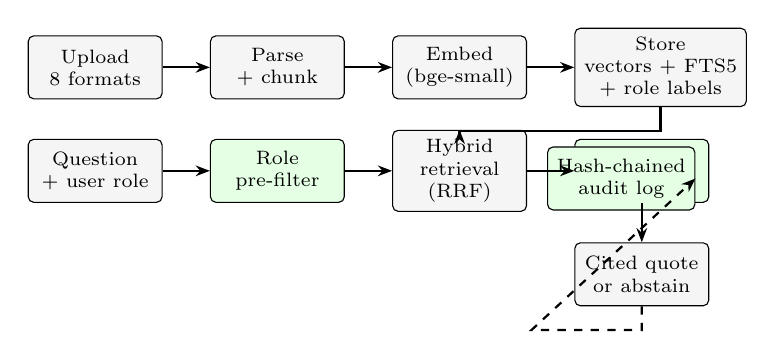
\begin{tikzpicture}[node distance=5mm and 6mm, every node/.style={font=\scriptsize},
  box/.style={draw, rounded corners=2pt, align=center, minimum height=8mm, minimum width=17mm, fill=gray!8},
  sec/.style={draw, rounded corners=2pt, align=center, minimum height=8mm, minimum width=17mm, fill=green!10},
  arr/.style={-{Stealth[length=1.8mm]}, thick}]
 \node[box] (up) {Upload\\8 formats};
 \node[box, right=of up] (parse) {Parse\\+ chunk};
 \node[box, right=of parse] (emb) {Embed\\(bge-small)};
 \node[box, right=of emb] (store) {Store\\vectors + FTS5\\+ role labels};
 \node[box, below=of up] (q) {Question\\+ user role};
 \node[sec, right=of q] (filt) {Role\\pre-filter};
 \node[box, right=of filt] (ret) {Hybrid\\retrieval\\(RRF)};
 \node[sec, right=of ret] (guard) {Answer\\guard};
 \node[box, below=of guard] (ans) {Cited quote\\or abstain};
 \node[sec, below=of store, xshift=-5mm] (audit) {Hash-chained\\audit log};
 \draw[arr] (up) -- (parse); \draw[arr] (parse) -- (emb); \draw[arr] (emb) -- (store);
 \draw[arr] (q) -- (filt); \draw[arr] (filt) -- (ret); \draw[arr] (ret) -- (guard); \draw[arr] (guard) -- (ans);
 \draw[arr] (store.south) -- ++(0,-3mm) -| (ret.north);
 \draw[arr, dashed] (ans.south) |- ++(-14mm,-3mm) -- (audit.east);
\end{tikzpicture}}
\caption{Knowledge Desk architecture. Green blocks are the security-relevant stages.}\label{fig:arch}
\end{figure}

\subsection{Parsing and chunking}
Every supported format is converted into an ordered list of blocks carrying a page (or slide/sheet) number, the nearest section heading, and a kind (text or table). PDF text, tables and headings are extracted with PyMuPDF, with repeated headers and footers removed; Word, Excel, CSV, PowerPoint (including speaker notes), HTML (boilerplate stripped), Markdown and plain text are handled by format-specific parsers, with character-encoding detection (UTF-8, UTF-16, Latin-1). Tables are rendered as Markdown so rows stay together. Text is packed by sentence into chunks of about 300 tokens with 50 tokens of overlap and never crosses a section boundary; tables are split by rows with the header repeated so every chunk is self-describing. The embedded text is prefixed with ``Title $>$ Section'' while the stored, cited text remains verbatim.

\subsection{Hybrid retrieval}
Passages are embedded with a 384-dimensional bge-small-en-v1.5 model \cite{xiao2023cpack} (int8-quantised ONNX, CPU); queries carry the model's retrieval instruction prefix. For a question $q$ and eligible passage set $\mathcal{E}$, the dense ranking orders $c\in\mathcal{E}$ by cosine similarity and the lexical ranking uses BM25 over a SQLite FTS5 index with Porter stemming. Each ranking is truncated to 24 items and fused by reciprocal rank fusion \cite{cormack2009rrf}:
\begin{equation}
\mathrm{RRF}(c)=\sum_{r\in\{\text{dense},\text{lex}\}}\frac{1}{60+\mathrm{rank}_r(c)},
\end{equation}
returning the top 10 passages.

\subsection{Role-aware pre-filtering}
Documents carry one of five classifications. A fixed lattice maps each to the roles allowed to read it (Table~\ref{tab:lattice}); notably, Manager and HR have disjoint confidential domains and Admin reads everything within its tenant. The set of allowed roles is stored on every chunk, and re-classifying a document relabels all of its chunks in the same database statement. The eligible set is
\begin{equation}
\mathcal{E}(u)=\{c : \mathrm{tenant}(c)=\mathrm{tenant}(u)\ \wedge\ \mathrm{ready}(c)\ \wedge\ \mathrm{role}(u)\in\mathrm{allowed}(c)\},
\end{equation}
computed \emph{inside the database query}; dense scoring and the full-text match only ever see $\mathcal{E}(u)$. After retrieval, the application re-checks every hit and fails closed (defence in depth).

\begin{table}[!t]
\caption{Access lattice: roles allowed to read each classification.}\label{tab:lattice}
\centering\small
\adjustbox{max width=\columnwidth}{\begin{tabular}{lcccc}
\toprule
Classification & Employee & Manager & HR & Admin\\
\midrule
Public, General Internal & \checkmark & \checkmark & \checkmark & \checkmark\\
Management & & \checkmark & & \checkmark\\
HR Confidential & & & \checkmark & \checkmark\\
Restricted & & & & \checkmark\\
\bottomrule
\end{tabular}}
\end{table}

\subsection{Evidence-first answer guard}
Let $T(\cdot)$ be the set of stemmed non-stop-word terms and $\mathrm{cov}(q,c)=|T(q)\cap T(c)|/|T(q)|$. A retrieved passage $c$ with dense cosine $s_c$ is \emph{supported} if
\begin{equation}
(s_c\ge\theta\ \wedge\ \mathrm{cov}(q,c)\ge 0.5)\ \vee\ \mathrm{cov}(q,c)\ge 0.8,\qquad \theta=0.55 .
\end{equation}
For up to three supported passages, the guard selects the (at most two) sentences, or the best-matching table rows with their header, that share the most terms with the question, and returns them verbatim with citations $[C_1],\dots$ linking to the source passage and page. If no passage is supported, a fixed fallback message is returned. No text is generated.

\subsection{Tamper-evident audit log}
Each question, answer, upload and administrative action is appended to a per-tenant chain. With $h_0=0^{64}$ and canonical record serialisation $r_i$,
\begin{equation}
h_i=\mathrm{SHA\text{-}256}(h_{i-1}\,\|\,r_i),
\end{equation}
and the database rejects \texttt{UPDATE} and \texttt{DELETE} on the log. Verification recomputes the whole chain. Authentication uses scrypt password hashes, short-lived signed session tokens and login rate limiting, and download links expire after 60 seconds and re-check the caller's role.

\subsection{Implementation}
The backend is FastAPI with an embedded SQLite store (vectors as float32 blobs, exact search in NumPy); the frontend is React. The system runs on a single machine, which suits small organisations and makes the evaluation below fully reproducible.

\section{Evaluation Method}\label{sec:eval}
\subsection{Research questions}
RQ1: which retriever (BM25, dense, hybrid) is most accurate and robust? RQ2: does role-aware pre-filtering prevent leakage, and does it differ from post-filtering or no filtering? RQ3: how reliable is the answer guard on unanswerable and near-duplicate questions? RQ4: are answers faithful to their sources? RQ5: do all formats survive parsing and remain retrievable? RQ6: does the audit chain detect tampering? RQ7: how does latency scale?

\subsection{Benchmark}
We generate a synthetic enterprise corpus because real corporate documents are confidential and unlabelled. It has 15 policy topics across the five classifications (e.g., leave and travel limits as General Internal, purchase limits and sales targets as Management, bonus and notice period as HR Confidential, project budgets as Restricted). Each document states several facts of the form ``\emph{\{entity\}} has \emph{\{value\}}'' with filler sentences; entities are combinations such as department\,$\times$\,office or grade\,$\times$\,track so that many documents are near-duplicates differing only in the entity. Each corpus has \NDocs{} documents, \NFacts{} facts and about \NChunks{} chunks. For every fact we create three questions: a template question (\emph{original}), a mildly reworded one, and a \emph{synonym} question that avoids the topic words of the source sentence (e.g., ``vacation allowance'' for ``annual leave'') but keeps the entity. A quarter of the entities of every topic is withheld from the corpus to form unanswerable questions. In total there are \NAnswerable{} answerable and \NUnanswerable{} unanswerable questions. We repeat everything on \NSeeds{} corpora generated with different seeds (different entity assignment, values and filler); the corpus \emph{structure} is the same, so the reported standard deviations underestimate variation across genuinely different collections.

All experiments run the real implementation: parser, chunker, int8 bge-small embeddings, SQLite store, retrieval and answer guard, on a consumer Windows laptop without a GPU.

\subsection{Metrics}
A retrieved chunk is \emph{gold} if it contains the verbatim sentence of the target fact. We report Recall@$k$ and mean reciprocal rank (MRR) over the top 10. An answer is \emph{correct} if it contains the gold sentence verbatim; \emph{wrong-entity} if the system answered but not with the gold sentence; and a \emph{false answer} if it answered an unanswerable question. A \emph{leak} occurs when a role receives, in the answer text or cited excerpts, any sentence of a fact that role may not read. For access control every answerable question is asked as each of the four roles, yielding \AuthPairs{} authorised and \UnauthPairs{} unauthorised question--role pairs per corpus.

\subsection{Compared systems}
\emph{No access control}: retrieval over the whole corpus. \emph{Post-filtering}: retrieve the top-10 over the whole corpus and drop passages the role cannot read. \emph{Pre-filtering} (ours): restrict candidates to $\mathcal{E}(u)$ before scoring. All three use the same answer guard.

\section{Results}\label{sec:results}
\subsection{RQ1: retrieval}
Table~\ref{tab:retr} and Fig.~\ref{fig:retr} show retrieval quality. On keyword-aligned questions BM25 is best (Recall@1 \RKwBmOne\%), ahead of hybrid (\RKwHyOne\%) and dense (\RKwDnOne\%), consistent with BM25 being a strong baseline on entity-heavy queries \cite{thakur2021beir}. On synonym questions the order changes: hybrid is best (\RSynHyOne\%), ahead of dense (\RSynDnOne\%) and BM25 (\RSynBmOne\%). Over all questions BM25 and hybrid are tied on Recall@1 (\ROverallBm\% versus \ROverallHy\%), both well above dense retrieval alone (\ROverallDn\%), while hybrid retrieval has the highest Recall@5 on synonym questions (\RSynHyFive\% versus \RSynBmFive\%). Hybrid retrieval is therefore never the worst retriever and is the most robust to how a user phrases a question, which motivates its use, but it does not dominate BM25 when queries repeat the document's own words.

\begin{table}[!t]
\caption{Retrieval ablation (mean $\pm$ std over \NSeeds{} corpora). R@$k$: Recall@$k$.}\label{tab:retr}
\centering\scriptsize
\adjustbox{max width=\columnwidth}{\begin{tabular}{lrrrr}
\toprule
Retriever & R@1 (\%) & R@3 (\%) & R@5 (\%) & MRR\\
\midrule
\multicolumn{5}{l}{\emph{Keyword-aligned queries}}\\
BM25 only & 63.4\,$\pm$\,1.9 & 96.7\,$\pm$\,0.5 & 99.9\,$\pm$\,0.1 & 0.791\,$\pm$\,0.012\\
Dense only & 53.1\,$\pm$\,1.8 & 78.2\,$\pm$\,1.3 & 87.5\,$\pm$\,1.4 & 0.675\,$\pm$\,0.013\\
Hybrid (RRF) & 60.0\,$\pm$\,0.9 & 89.2\,$\pm$\,1.3 & 96.2\,$\pm$\,0.6 & 0.752\,$\pm$\,0.009\\
\multicolumn{5}{l}{\emph{Synonym queries}}\\
BM25 only & 46.2\,$\pm$\,1.4 & 73.0\,$\pm$\,0.6 & 81.3\,$\pm$\,0.7 & 0.605\,$\pm$\,0.009\\
Dense only & 48.6\,$\pm$\,0.9 & 72.6\,$\pm$\,2.1 & 81.6\,$\pm$\,0.8 & 0.628\,$\pm$\,0.009\\
Hybrid (RRF) & 52.7\,$\pm$\,0.7 & 79.8\,$\pm$\,1.6 & 89.6\,$\pm$\,0.7 & 0.680\,$\pm$\,0.004\\
\bottomrule
\end{tabular}
}
\end{table}

\begin{figure}[!t]
\centering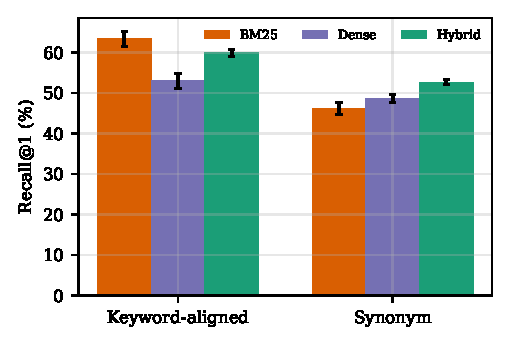
\includegraphics[width=.8\columnwidth]{figures/retrieval}
\caption{Recall@1 by retriever and query style (error bars: std over corpora).}\label{fig:retr}
\end{figure}

\subsection{RQ2: access control}
Table~\ref{tab:acc} compares the three systems. Without access control, restricted content appeared in the cited answer for \LeakNoAcl\% of unauthorised questions, and a restricted passage was among the top five results for \TopFiveNoAcl\% of them. Both post-filtering and pre-filtering produced no leaks (\LeakPost\% and \LeakPre\%), and their accuracy on authorised questions was practically identical (\AccPost\% versus \AccPre\%; \AccNoAcl\% without access control, whose authorised-question accuracy is not meaningfully different). The top-$k$ sweep in Fig.~\ref{fig:k} shows that pre-filtering is slightly better at very small $k$ ($k{=}1$: \KOnePre\% versus \KOnePost\%), as expected when restricted passages can crowd out authorised ones in a short post-filtered list, but the difference is below one percentage point on this benchmark. We therefore \emph{do not} claim an accuracy advantage for pre-filtering. Its advantage is structural: restricted passages are never loaded, scored or ranked for an unauthorised user, so correctness of the security property does not depend on $k$, on the filter being applied after every ranking path, or on what intermediate components log.

An additional effect appears for unauthorised questions: with pre-filtering the system abstained in \AbstPre\% of cases versus \AbstPost\% for post-filtering. The remainder are not leaks, but answers built from \emph{readable near-duplicate} documents about a different entity (silent substitution), which the guard analysed in Section~\ref{sec:guard} only partly addresses.

\begin{table}[!t]
\caption{Access control comparison (mean $\pm$ std over corpora).}\label{tab:acc}
\centering\scriptsize
\adjustbox{max width=\columnwidth}{\begin{tabular}{lrrr}
\toprule
System & Correct (\%) & Leaked answers (\%) & Top-5 exposure (\%)\\
\midrule
No access control & 63.9\,$\pm$\,1.1 & 87.1\,$\pm$\,0.0 & 100.0\,$\pm$\,0.0\\
Post-filtering & 64.3\,$\pm$\,1.1 & 0.0\,$\pm$\,0.0 & 0.0\,$\pm$\,0.0\\
Pre-filtering (ours) & 64.4\,$\pm$\,1.2 & 0.0\,$\pm$\,0.0 & 0.0\,$\pm$\,0.0\\
\bottomrule
\end{tabular}
}
\end{table}

\begin{figure}[!t]
\centering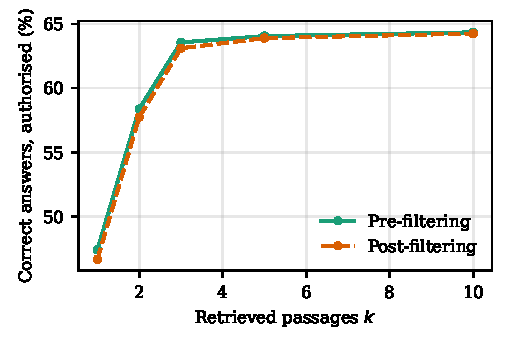
\includegraphics[width=.8\columnwidth]{figures/ksweep}
\caption{Accuracy on authorised questions versus number of retrieved passages $k$.}\label{fig:k}
\end{figure}

\subsection{RQ3: answer guard and entity-span guard}\label{sec:guard}
The deployed guard (Eq.~3) is permissive on near-duplicate corpora (Table~\ref{tab:guard}). It answers correctly \GStdCorr\% of the time but returns a wrong-entity answer for \GStdWrong\% of answerable questions and a false answer for \GStdFalse\% of unanswerable ones. The reason is that term coverage is computed over a whole chunk, which contains several entities' sentences; a question about an absent entity still has all its topic words present. Requiring each quoted sentence to cover most of the question's terms helps only at the price of rejecting legitimate synonym questions (sentence coverage $\ge0.8$: correct \GCovEightCorr\%, wrong entity \GCovEightWrong\%, false \GCovEightFalse\%; at $0.9$ correct answers fall to \GCovNineCorr\% and to \GCovNineSynCorr\% for synonym questions), because a lexical criterion cannot tell an entity mismatch from a synonym.

We therefore test an \emph{entity-span guard}: extract the named-entity spans of the question (maximal runs of capitalised or coded tokens such as ``Engineering (Bengaluru)'' or ``G5-technical'') and require each span to appear verbatim in the quoted text. It reduces wrong-entity answers to \GEAllWrong\% and false answers to \GEAllFalse\% without reducing the share of correct answers (\GEAllCorr\%, identical to the deployed guard): the answers it removes become abstentions (\GEAllAbst\% of answerable questions versus \GSAllAbst\%), which is the intended trade (Table~\ref{tab:guard}, Fig.~\ref{fig:guard}); on synonym questions it keeps \GESynCorr\% correct, versus \GCovNineSynCorr\% for the strict coverage guard. In the access-control setting it lowers silent substitution (answers to unauthorised questions built from readable documents) from \SubstS\% to \SubstE\%, though it does not eliminate it, and on synonym questions it still lets through \GESynFalse\% false answers.

\begin{table}[!t]
\caption{Answer guard comparison on all questions (mean $\pm$ std).}\label{tab:guard}
\centering\scriptsize
\adjustbox{max width=\columnwidth}{\begin{tabular}{lrrr}
\toprule
Guard & Correct (\%) & Wrong entity (\%) & False answers (\%)\\
\midrule
Standard guard (deployed) & 66.9\,$\pm$\,0.9 & 21.5\,$\pm$\,1.0 & 80.6\,$\pm$\,0.5\\
Sentence coverage $\geq 0.8$ & 49.7\,$\pm$\,0.8 & 7.0\,$\pm$\,0.5 & 31.1\,$\pm$\,0.5\\
Entity-span guard (proposed) & 66.9\,$\pm$\,0.9 & 1.6\,$\pm$\,0.4 & 7.7\,$\pm$\,1.3\\
\bottomrule
\end{tabular}
}
\end{table}

\begin{table}[!t]
\caption{Guards by question style.}\label{tab:guardtype}
\centering\scriptsize
\adjustbox{max width=\columnwidth}{\begin{tabular}{llrrr}
\toprule
Queries & Guard & Correct (\%) & Wrong entity (\%) & False answers (\%)\\
\midrule
Keyword-aligned & Standard & 77.0\,$\pm$\,1.3 & 23.0\,$\pm$\,1.3 & 100.0\,$\pm$\,0.0\\
Keyword-aligned & Sent. cov. 0.8 & 74.5\,$\pm$\,1.2 & 10.5\,$\pm$\,0.8 & 62.1\,$\pm$\,1.1\\
Keyword-aligned & Entity-span & 77.0\,$\pm$\,1.3 & 0.4\,$\pm$\,0.3 & 2.5\,$\pm$\,0.4\\
Synonym & Standard & 46.8\,$\pm$\,0.3 & 18.4\,$\pm$\,0.8 & 61.1\,$\pm$\,1.1\\
Synonym & Sent. cov. 0.8 & 0.0\,$\pm$\,0.0 & 0.0\,$\pm$\,0.0 & 0.0\,$\pm$\,0.0\\
Synonym & Entity-span & 46.8\,$\pm$\,0.3 & 4.2\,$\pm$\,0.7 & 12.8\,$\pm$\,2.3\\
\bottomrule
\end{tabular}
}
\end{table}

\begin{figure}[!t]
\centering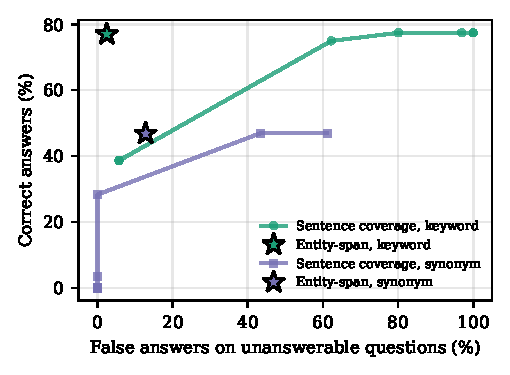
\includegraphics[width=.85\columnwidth]{figures/guard_tradeoff}
\caption{Correct answers versus false answers. Lines: sentence-coverage threshold sweep; stars: entity-span guard.}\label{fig:guard}
\end{figure}

\subsection{RQ4: faithfulness}
Across \FaithLines{} answer lines produced on \NSeeds{} corpora, \FaithVerbatim{} were verbatim substrings of retrieved passages, as the design implies. This guarantees that the system never invents text, but, as RQ3 shows, it does not guarantee correct answers.

\subsection{RQ5: file formats}
To isolate parsing, the same facts were written into eight formats and sent through the real parsers (Table~\ref{tab:fmt}). Every fact was recovered verbatim in every format (extraction \FmtMinExtract\%), so parsing loses no content. Retrieval quality was similar for seven formats (Recall@3 \FmtOthMinThree\%--\FmtOthMaxThree\%) and lower for Markdown (\FmtMdThree\%). Markdown headings split each document into more chunks (\FmtMdChunks\ versus about \FmtOthChunks\ in total), which plausibly makes near-duplicate passages harder to separate; we did not test this explanation separately.

\begin{table}[!t]
\caption{Format robustness (same facts, eight formats).}\label{tab:fmt}
\centering\scriptsize
\adjustbox{max width=\columnwidth}{\begin{tabular}{lrrrr}
\toprule
Format & Facts & Extracted (\%) & R@1 (\%) & R@3 (\%)\\
\midrule
Markdown & 80 & 100.0 & 53.8 & 82.5\\
Plain text & 80 & 100.0 & 50.0 & 91.2\\
HTML & 80 & 100.0 & 48.8 & 91.2\\
Word (.docx) & 80 & 100.0 & 47.5 & 91.2\\
Excel (.xlsx) & 80 & 100.0 & 50.0 & 88.8\\
CSV & 80 & 100.0 & 51.2 & 92.5\\
PowerPoint (.pptx) & 80 & 100.0 & 56.2 & 88.8\\
PDF & 80 & 100.0 & 50.0 & 91.2\\
\bottomrule
\end{tabular}
}
\end{table}

\subsection{RQ6: audit log}
We appended 1{,}000 and 5{,}000 records and then applied 40 random tampering attempts at each size, cycling over editing a record, deleting a record, and breaking a hash link, restoring the log after each. All \AuditDetected{} of \AuditTrials{} attempts were detected, with no false alarm on the untouched chain; verifying 5{,}000 records took \AuditVerifyFive\,s (Table~\ref{tab:audit}).

\begin{table}[!t]
\caption{Audit-chain verification and tamper detection.}\label{tab:audit}
\centering\scriptsize
\adjustbox{max width=\columnwidth}{\begin{tabular}{rrr}
\toprule
Records & Verify time (s) & Tampering detected\\
\midrule
1,000 & 0.03 & 40/40\\
5,000 & 0.12 & 40/40\\
\bottomrule
\end{tabular}
}
\end{table}

\subsection{RQ7: scalability}
Fig.~\ref{fig:scale} shows retrieval latency against index size (random vectors with real query texts, so only latency is meaningful). With exact search, median latency was \LatOneKEmpPFifty\,ms at 1{,}000 passages and \LatFiftyKEmpPFifty\,ms at 50{,}000 for an employee (\LatFiftyKAdmPFifty\,ms for an administrator, who has more eligible passages; 95th percentile \LatFiftyKAdmPNinetyFive\,ms). Latency grows roughly linearly with the eligible set, which is acceptable for departmental collections but would require approximate indexes \cite{malkov2018hnsw,johnson2019faiss} partitioned by role at larger scale.

\begin{figure}[!t]
\centering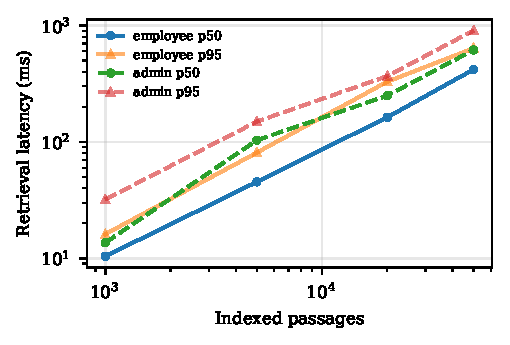
\includegraphics[width=.8\columnwidth]{figures/scaling}
\caption{Retrieval latency versus indexed passages (exact search).}\label{fig:scale}
\end{figure}

\section{Discussion and Limitations}\label{sec:discussion}
\textbf{What the results support.} Role-aware retrieval removed leakage in our tests, and a retrieval stage without it leaks readily. Hybrid retrieval is a robust default but not a universal win. The audit chain reliably exposes edits made without recomputing hashes. \textbf{What they do not support.} They do not show that pre-filtering is more \emph{accurate} than post-filtering. They do not show that the entity-span guard generalises: it exploits a convention (named entities are capitalised or coded tokens) that our own benchmark follows, so it needs validation on real documents. Our guard evaluation also tunes nothing on a held-out set, because all numbers are computed on generated corpora of identical structure.

\textbf{Faithful is not correct.} Eliminating generation removes invented text but not wrong answers: with the deployed guard roughly one in five answerable questions received a verbatim but wrong-entity sentence. Evaluation protocols for RAG should report both faithfulness and entity-level correctness, particularly where near-duplicate documents are common.

\textbf{Threat model.} We consider authenticated users with different roles who submit arbitrary questions. We do not defend against a compromised server, an attacker with write access to the database file, or timing and abstention side channels. A hash chain stored with the data can be recomputed by someone who can rewrite the whole database, so real tamper-evidence requires periodically anchoring the latest hash outside the system \cite{crosby2009tamper}.

\textbf{Validity threats.} The benchmark is synthetic and templated; the author of the system also wrote the benchmark; one embedding model and one chunking configuration were evaluated; scalability results use random vectors; there is no user study; and there is no generative baseline, so we make no claim about relative hallucination rates against LLM-based RAG. Scanned PDFs require OCR, which is not available in the hosted configuration.

\section{Conclusion and Future Work}
We presented Knowledge Desk, a document question-answering system that never generates text, and evaluated its real implementation. Role-aware filtering prevented all leakage, hybrid retrieval was the most robust retriever, every audit tampering attempt was detected, and an entity-span guard markedly reduced false and wrong-entity answers. The main lessons are negative or cautionary: pre-filtering is justified by structure rather than accuracy, and faithful extraction still yields wrong answers on near-duplicate documents. Future work includes a citation-constrained generation layer on top of the guarded retrieval; evaluation on real public policy corpora with human judgements; role-partitioned approximate indexes; learned entity-aware abstention; and external anchoring of the audit chain.

\section*{Acknowledgment}
[Acknowledgement of the industry contact who proposed the problem statement and reviewed the prototype: to be included only in wording approved by that person.] The authors thank their faculty mentor for guidance.

\section*{Availability}
The source code, benchmark generator and experiment scripts are in the project repository: \url{https://github.com/apranav1711-byte/knowledge-desk}.

\bibliographystyle{IEEEtran}
\bibliography{refs/refs}

\end{document}
